% !TeX program = xelatex
% !TeX encoding = UTF-8 Unicode
% !BIB program = biber

\documentclass[ieee,english]{slides}

\usepackage{mathtools}

\DeclareMathOperator*{\argmax}{arg\,max}
\DeclareMathOperator*{\argmin}{arg\,min}
\newcommand{\norm}[1]{\left\lVert#1\right\rVert}
\newcommand{\cmark}{\ding{51}}
\newcommand{\xmark}{\ding{55}}
\newcommand{\adj}{\textrm{adj}}
\newcommand{\tr}{^{\top}}
\renewcommand{\bar}[1]{\overline{#1}}
\newcommand{\ubar}[1]{\underline{#1}}

\title{Zero-Dynamics attack detection with Time-Scale Observer}

\addauthor{Álan Crístoffer e Sousa}{alan.e-sousa@univ-reims.fr}

\setorientador{Nadhir Messai}
\addcoorientador{Noureddine Manamanni}

\setdepartamento{CReSTIC}
\seteixodeformacao{Automation and Signal Processing}

\setlocal{Reims}
\setano{2023}
\setmes{February}

\preamble{}
\input{colors}

\addbibresource{bibliothek.bib}
\graphicspath{{imgs/}}%

\newcommand{\y}{\textcolor{flame}{\ensuremath{y(t)}}}
\newcommand{\z}{\textcolor{red}{\ensuremath{z(t)}}}
\newcommand{\w}{\textcolor{auburn}{\ensuremath{w(t)}}}
\newcommand{\hz}{\textcolor{red}{\ensuremath{\hat{z}(t)}}}
\newcommand{\dw}{\textcolor{auburn}{\ensuremath{\dot{w}(t)}}}
\newcommand{\mN}{\textcolor{frenchblue}{\ensuremath{N}}}
\newcommand{\mJ}{\textcolor{frenchblue}{\ensuremath{J}}}
\newcommand{\mH}{\textcolor{frenchblue}{\ensuremath{H}}}
\newcommand{\mE}{\textcolor{frenchblue}{\ensuremath{E}}}

\newcommand{\cubar}[1]{\textcolor{frenchblue}{\ubar{#1}}}
\newcommand{\cbar}[1]{\textcolor{flame}{\bar{#1}}}
\newcommand{\abs}[1]{\left\lVert#1\right\rVert}

\begin{document}
\maketitle{}

\begin{slide}{Index}
  \begin{minipage}[t][0.4\textheight][t]{0.45\textwidth}
    \tableofcontents[sections={1-4}]
  \end{minipage}
  \begin{minipage}[t][0.4\baselineskip][t]{0.45\textwidth}
    \tableofcontents[sections={5-}]
  \end{minipage}
  \vfill\null{}
\end{slide}

% !TeX root = document.tex
% !TeX encoding = UTF-8 Unicode

\section{Zero-Dynamics Attack}%
\label{sec:zda}

\subsection{Introduction}%
\label{subsec:ts-introduction}

\begin{slide}{Zero-Dynamics Attack}
  \begin{columns}[c]
    \begin{column}{0.48\textwidth}
      The attacker changes the control signal in a specific direction, taking
      advantage of the system's transmission zeros to change the system's states
      without affecting the system's output.
      \includegraphics[width=\linewidth]{ct-system}
    \end{column}%
    \hfill%
    \begin{column}{0.48\textwidth}
      \begin{align}
        \dot{x}       & = Ax + Bu                                       \\
        y             & = Cx + Du                                       \\
        \nonumber                                                       \\
        P(s)          & = \begin{bmatrix}
                            sI-A & -B \\
                            C    & D
                          \end{bmatrix},                                \\
        P(s_{0})z_{0} & = 0.                                            \\
        z_{0}         & = \begin{bmatrix} x_{0} \\ a_{0} \end{bmatrix}, \\
        a(t)          & = a_{0}e^{s_{0}t},                              \\
        \tilde{u}(t)  & =u(t) + a(t).
      \end{align}
    \end{column}%
  \end{columns}
\end{slide}

\subsection{Bibliography Review}%
\label{subsec:literature}

\begin{slide}{Current Literature Solutions}
  \begin{columns}[c]
    \begin{column}{0.48\textwidth}
      Current detection schemes in the literature:\\~\\
      \begin{itemize}
        \item Generalized Zero-Order Holders \\
              \textcolor{gray}{\textcite{kim.ryu.ea:zero-dynamics,shim.back.ea:zero-dynamics}}
        \item Modified system models \\
              \textcolor{gray}{\textcite{baniamerian.khorasani.ea:monitoring}}
        \item Topology change \\
              \textcolor{gray}{\textcite{mao.jafarnejadsani.ea:novel}}
      \end{itemize}
    \end{column}%
    \hfill%
    \begin{column}{0.48\textwidth}
      \begin{figure}[ht!]
        \centering
        \resizebox{0.6\linewidth}{!}{%
          \begin{tikzpicture}[node distance=1cm,block/.style={align=center,draw,shape=rectangle,very thick,minimum height=2em, minimum width=3em},>=stealth]
            \node (C) [block]                             {Controller};
            \node (G) [block,above=1.5cm of C]            {System};
            \node (H) [block,below=of C]                  {Time-Scale Observer};
            \node (u) [above left=0.5cm and 1cm of C]     {\(u(t)\)};
            \node (y) [above right=0.5cm and 1cm of C]    {\(y(t)\)};
            \node     [draw,rectangle,dashed,fit=(u) (y)] {Network};

            \draw [->,thick] (C) -| (u) |- (G);
            \draw [->,thick] (G) -| (y) |- (C);
            \draw [->,thick] (u) |- (H);
            \draw [->,thick] (y) |- (H);
          \end{tikzpicture}%
        }
        \caption{Conventional Observer's block diagram}%
      \end{figure}    \end{column}%
  \end{columns}
\end{slide}

\begin{slide}{Current Literature Solutions}
  \begin{columns}[c]
    \begin{column}{0.48\textwidth}
      Current detection schemes in the literature:\\~\\
      \begin{itemize}
        \item Generalized Zero-Order Holders \\
              \textcolor{gray}{\textcite{kim.ryu.ea:zero-dynamics,shim.back.ea:zero-dynamics}}
        \item Modified system models \\
              \textcolor{gray}{\textcite{baniamerian.khorasani.ea:monitoring}}
        \item Topology change \\
              \textcolor{gray}{\textcite{mao.jafarnejadsani.ea:novel}}
      \end{itemize}
    \end{column}%
    \hfill%
    \begin{column}{0.48\textwidth}
      \begin{figure}[ht!]
        \centering
        \resizebox{0.6\linewidth}{!}{%
          \begin{tikzpicture}[node distance=1cm,block/.style={align=center,draw,shape=rectangle,very thick,minimum height=2em, minimum width=3em},>=stealth]
            \node (C) [block]                             {Controller};
            \node (G) [block,above=1.5cm of C]            {System};
            \node (H) [block,above=of G]                  {Time-Scale Observer};
            \node (u) [above left=0.5cm and 1cm of C]     {\(u(t)\)};
            \node (y) [above right=0.5cm and 1cm of C]    {\(y(t)\)};
            \node     [draw,rectangle,dashed,fit=(u) (y)] {Network};

            \draw [->,thick] (C) -| (u) |- (G);
            \draw [->,thick] (G) -| (y) |- (C);
            \draw [->,thick] (u) |- (H);
            \draw [->,thick] (y) |- (H);
          \end{tikzpicture}%
        }
        \caption{Proposed Observer's block diagram}%
      \end{figure}
    \end{column}%
  \end{columns}
\end{slide}

% !TeX root = document.tex
% !TeX encoding = UTF-8 Unicode

\section{Time-Scale Systems}%
\label{sec:ts-systems}

\subsection{Time Scale Calculus}%
\label{subsec:ts-calculus}

\begin{slide}{Time-Scale Calculus}
  \begin{columns}[c]
    \begin{column}{0.48\textwidth}
      \begin{itemize}
        \item Unifies the continuous- and discrete-time calculi.
        \item Uses the so-called delta-derivative (\(\Delta\)-derivative).
        \item Exists for different time-sets, not only the continuous and
              discrete case.
      \end{itemize}
      \begin{figure}[ht!]
        \centering
        \includegraphics[width=0.6\linewidth]{ts-jump}
        \caption{Time-Scale jump operators. Source: \url{https://shorturl.at/bcJY1}}%
      \end{figure}
    \end{column}%
    \hfill%
    \begin{column}{0.48\textwidth}
      \begin{equation}
        \mathbb{T} = h\mathbb{Z} | \mathbb{R} | \mathbb{T}_{\textrm{iso}}
      \end{equation}
      %
      \begin{align}
        \textrm{forward:~}  & \sigma(t) = \inf\{\tau\in\mathbb{T}|\tau>t\}, \\
        \textrm{backward:~} & \rho(t) = \sup\{\tau\in\mathbb{T}|\tau<t\}.
      \end{align}
      %
      \begin{equation}
        \mu(t) = \sigma(t)-t \leftarrow \textrm{graininess}
      \end{equation}
      %
      \begin{equation}
        f(\sigma(t)) = f(t) + \mu(t)f^{\Delta}(t).
      \end{equation}
      %
      \begin{equation}
        f^{\Delta}(t) = \lim_{\delta\rightarrow{}\mu(t)}\frac{f(t+\delta)-f(t)}{\delta}.
      \end{equation}
    \end{column}%
  \end{columns}
\end{slide}

\begin{slide}{Time-Scale System}
  \begin{columns}[c]
    \begin{column}{0.38\textwidth}
      \begin{itemize}
        \item Allows to evolve the system with arbitrary sampling-times.
        \item Has it own stability criteria based on the Hilger's circle.
      \end{itemize}
    \end{column}%
    \hfill%
    \begin{column}{0.58\textwidth}
      \begin{align}
        \textrm{Continuous-Time System} & \nonumber                                                                 \\
        \dot{x}(t)                      & = \mathcal{A}x(t) + \mathcal{B}u(t),                                      \\
        y(t)                            & = Cx(t) + Du(t),                                                          \\
        \textrm{Time-Scale System}      & \nonumber                                                                 \\
        x^{\Delta}(t)                   & = A(\mu(t))x(t) + B(\mu(t))u(t),                                          \\
        y(t)                            & = Cx(t) + Du(t),                                                          \\
        \phantom{1}                     & \phantom{1}                                 \nonumber                     \\
        A(\mu(t))                       & = \frac{e^{\mathcal{A}\mu(t)}-I}{\mu(t)},                                 \\
        B(\mu(t))                       & = \int_{0}^{\mu(t)}\frac{e^{(\mu(t)-s)\mathcal{A}}}{\mu(t)}\mathcal{B}ds.
      \end{align}
    \end{column}%
  \end{columns}
\end{slide}

\begin{slide}{Stability Criteria}
  \begin{columns}[c]
    \begin{column}{0.48\textwidth}
      The system is stable if all of it's poles are within the Hilger's circle,
      defined as a the circle centered at \((-\frac{1}{\mu}, 0)\) and with
      radius \(\frac{1}{\mu}\).

      Note that the circle changes with the sampling-time (\(\mu\)).

      \begin{equation}
        \mathcal{H}_{\mu} \coloneqq \left\{ z \in \mathbb{C} : \abs{z + \frac{1}{\mu}} < \frac{1}{\mu} \right\}
      \end{equation}
    \end{column}%
    \hfill%
    \begin{column}{0.48\textwidth}
      \begin{figure}[ht!]
        \centering
        \resizebox{\linewidth}{!}{%
          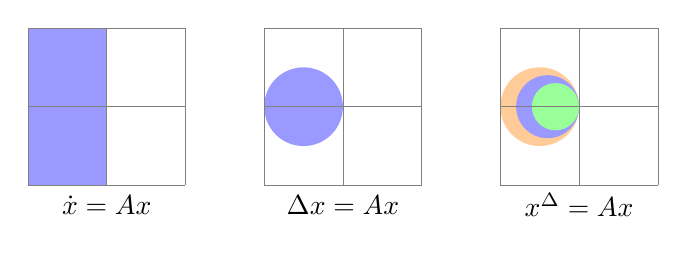
\begin{tikzpicture}
            \fill [blue!40!white]           (0, 0) rectangle (1, 2);
            \draw [step=1cm,gray,very thin] (0, 0) grid      (2, 2);
            \node at (1, -0.25) {\(\dot{x}=Ax\)};

            \fill [blue!40!white]           (3.5, 1) circle (0.5);
            \draw [step=1cm,gray,very thin] (3, 0)   grid   (5, 2);
            \node at (4, -0.25) {\(\Delta{}x=Ax\)};

            \fill [orange!40!white]         (6.5, 1) circle (0.5);
            \fill [blue!40!white]           (6.6, 1) circle (0.4);
            \fill [green!40!white]          (6.7, 1) circle (0.3);
            \draw [step=1cm,gray,very thin] (6, 0)   grid   (8, 2);
            \node at (7, -0.25) {\(x^{\Delta{}}=Ax\)};
          \end{tikzpicture}%
        }
        \caption{Different stability regions}%
      \end{figure}
    \end{column}%
  \end{columns}
\end{slide}

% !TeX root = document.tex
% !TeX encoding = UTF-8 Unicode

\subsection{Hypothesis}%
\label{subsec:hypothesis}

\begin{slide}{Hypothesis}
  \begin{enumerate}
    \item The system is observable;\label{item:hypo1}
    \item The system's poles are real;\label{item:hypo2}
  \end{enumerate}
\end{slide}

\subsection{Observer Synthesis}%
\label{subsec:ts-observer-synthesis}

\begin{slide}{Observer Synthesis}
  \begin{columns}[c]
    \begin{column}{0.55\textwidth}
      \begin{itemize}
        \item Taking into consideration Hypothesis~\ref{item:hypo1}
      \end{itemize}
      \begin{align}
        x^{\Delta} & = Ax + Bu, \\
        y          & = Cx,
      \end{align}
      %
      \begin{gather}
        V = x\tr{}Px
      \end{gather}
      %
      \begin{gather}
        x(\sigma(t)) = x(t) + \mu(t)x^{\Delta}(t).
      \end{gather}
      %
      \begin{gather}
        PA + A\tr{}P + \mu{}A\tr{}PA \prec{} 0 \\
        P \succ{} 0
      \end{gather}
    \end{column}%
    \hfill%
    \begin{column}{0.55\textwidth}
      \begin{equation}
        x^{\Delta} = Ax + Bu + L(y - Cx).
      \end{equation}
      %
      \begin{gather}
        \begin{bmatrix}
          M     & (PA - ZC)  \\
          \star & -\mu^{-1}P
        \end{bmatrix} \prec{} 0,  \\
        M = PA + A\tr{}P - ZC - C\tr{}Z\tr{}.
      \end{gather}
      %
      \begin{equation}
        Z = PL.
      \end{equation}
    \end{column}%
  \end{columns}
\end{slide}

\begin{slide}{LPV Observer}
  \begin{columns}[c]
    \begin{column}{0.55\textwidth}
      The time-scale system is nonlinear and parameter-varying since it's \(A\)
      matrix is
      %
      \begin{equation}
        A(\mu(t)) = \frac{e^{\mathcal{A}\mu(t)}-I}{\mu(t)},
      \end{equation}
      %
      which allows the application of sector-decomposition.
    \end{column}%
    \hfill%
    \begin{column}{0.55\textwidth}
      For a non-linear function \(f(\rho):\mathbb{R}\rightarrow\mathbb{R}\), given
      \(\rho\in[\ubar{\rho}, \bar{\rho}]\), then
      %
      \begin{equation}
        f(\rho) = \alpha_{1}(\rho)\ubar{f} + \alpha_{2}(\rho)\bar{f}
      \end{equation}
      %
      if
      %
      \begin{align}
        \bar{f}          & = \sup{f(\rho)},                             \\
        \ubar{f}         & = \inf{f(\rho)},                             \\
        \nonumber                                                       \\
        \alpha_{1}(\rho) & = \frac{\bar{f}-f(\rho)}{\bar{f}-\ubar{f}},  \\
        \alpha_{2}(\rho) & = \frac{f(\rho)-\ubar{f}}{\bar{f}-\ubar{f}}.
      \end{align}
    \end{column}%
  \end{columns}
\end{slide}

\begin{slide}{Convexity and Majorization}
  \begin{columns}[c]
    \begin{column}{0.55\textwidth}
      Taking into consideration Hypothesis~\ref{item:hypo2}.
      %
      \begin{equation}
        f(\sum_{i}\alpha_{i}x_{i}) \preceq \sum_{i}\alpha_{i}f(x_{i}),
      \end{equation}
    \end{column}%
    \hfill%
    \begin{column}{0.55\textwidth}
      \begin{itemize}
        \item Convexity is not globally defined for complex numbers;
        \item Convexity is not globally defined for matrices;
      \end{itemize}
    \end{column}%
  \end{columns}
\end{slide}

\begin{slide}{LMI for the LPV Case}
  \begin{equation}
    V = \begin{bmatrix}
      M(\sum_{i=0}^{1}\gamma_{i}(\mu)\mu_{i},\sum_{i=0}^{1}\beta_{i}(\mu)(\frac{1}{\mu})_{i}) & PA(\sum_{i=0}^{1}\gamma_{i}(\mu)\mu_{i}) - Z(\cdot)C \\
      \star                                                                                   & -\sum_{i=0}^{1}\beta_{i}(\mu)(\frac{1}{\mu})_{i}P
    \end{bmatrix},
  \end{equation}
  \begin{equation}
    V \preceq \begin{bmatrix}
      \sum_{i=0}^{1}\gamma_{i}(\mu)\cdot\sum_{i=0}^{1}\beta_{i}(\mu)(\frac{1}{\mu})_{i}\cdot{}M_{i,j} & P\sum_{i=0}^{1}\gamma_{i}(\mu)A_{i} - Z(\cdot)C   \\
      \star                                                                                           & -\sum_{i=0}^{1}\beta_{i}(\mu)(\frac{1}{\mu})_{i}P
    \end{bmatrix},
  \end{equation}
\end{slide}

\begin{slide}{LMI Recapitulation}
  \begin{columns}[c]
    \begin{column}{0.55\textwidth}
      \begin{align}
        \hat{x}^{\Delta} & = A(\mu)\hat{x} + B(\mu)u - L(\mu)(y - C\hat{x}),                                                                                                         \\
        L(\mu)           & = \sum_{i=0}^{3}\alpha_{i}(\mu)L_{i},                                                                                                                     \\
        \alpha_{0}(\mu)  & = \textcolor{frenchblue}{\frac{\bar{\mu}^{-1}-\mu^{-1}}{\bar{\mu}^{-1}-\ubar{\mu}^{-1}}}  \textcolor{flame}{\frac{\bar{\mu}-\mu}{\bar{\mu}-\ubar{\mu}}},  \\
        \alpha_{1}(\mu)  & = \textcolor{frenchblue}{\frac{\mu^{-1}-\ubar{\mu}^{-1}}{\bar{\mu}^{-1}-\ubar{\mu}^{-1}}} \textcolor{flame}{\frac{\bar{\mu}-\mu}{\bar{\mu}-\ubar{\mu}}},  \\
        \alpha_{2}(\mu)  & = \textcolor{frenchblue}{\frac{\bar{\mu}^{-1}-\mu^{-1}}{\bar{\mu}^{-1}-\ubar{\mu}^{-1}}}  \textcolor{flame}{\frac{\mu-\ubar{\mu}}{\bar{\mu}-\ubar{\mu}}}, \\
        \alpha_{3}(\mu)  & = \textcolor{frenchblue}{\frac{\mu^{-1}-\ubar{\mu}^{-1}}{\bar{\mu}^{-1}-\ubar{\mu}^{-1}}} \textcolor{flame}{\frac{\mu-\ubar{\mu}}{\bar{\mu}-\ubar{\mu}}},
      \end{align}
    \end{column}%
    \hfill%
    \begin{column}{0.55\textwidth}
      \begin{align}
                 & \begin{bmatrix}
                     M(\cubar{\mu},0) & PA(\cubar{\mu}) - Z_{0}C \\
                     \star            & -\frac{1}{\cubar{\mu}}P
                   \end{bmatrix} \prec{} 0,  \\
                 & \begin{bmatrix}
                     M(\cbar{\mu},1) & PA(\cbar{\mu}) - Z_{1}C \\
                     \star           & -\frac{1}{\cubar{\mu}}P
                   \end{bmatrix} \prec{} 0,    \\
                 & \begin{bmatrix}
                     M(\cubar{\mu},2) & PA(\cubar{\mu}) - Z_{2}C \\
                     \star            & -\frac{1}{\cbar{\mu}}P
                   \end{bmatrix} \prec{} 0, \\
                 & \begin{bmatrix}
                     M(\cbar{\mu},3) & PA(\cbar{\mu}) - Z_{3}C \\
                     \star           & -\frac{1}{\cbar{\mu}}P
                   \end{bmatrix} \prec{} 0,   \\
        M(\mu,i) & = PA(\mu) + A(\mu)\tr{}P - Z_{i}C - C\tr{}Z_{i}\tr,      \\
        L_{i}    & = P^{-1}Z_{i}.
      \end{align}
    \end{column}%
  \end{columns}
\end{slide}

% !TeX root = document.tex
% !TeX encoding = UTF-8 Unicode

\subsection{Results}%
\label{subsec:ts-results}

\begin{slide}{Observer}
  \begin{columns}[c]
    \begin{column}{0.55\textwidth}
      \begin{align}
        \mathcal{A}    & = \begin{bmatrix}
                             0 & 0 & 0 & 0 & -120 \\
                             1 & 0 & 0 & 0 & -274 \\
                             0 & 1 & 0 & 0 & -225 \\
                             0 & 0 & 1 & 0 & -85  \\
                             0 & 0 & 0 & 1 & -15
                           \end{bmatrix},             \\
        \mathcal{B}    & =\begin{bmatrix}
                            1 \\ 0 \\ 0 \\ 0 \\ 0
                          \end{bmatrix},
        \mathcal{C} = \begin{bmatrix}
                        0 \\ 0 \\ 0 \\ 66 \\ -1056
                      \end{bmatrix}^{\top},
        \mathcal{D} = 0                                     \\
        \textrm{poles} & = \{-1, -2, -3, -4, -5\}
      \end{align}
    \end{column}%
    \hfill%
    \begin{column}{0.55\textwidth}
      \begin{figure}[ht!]
        \centering
        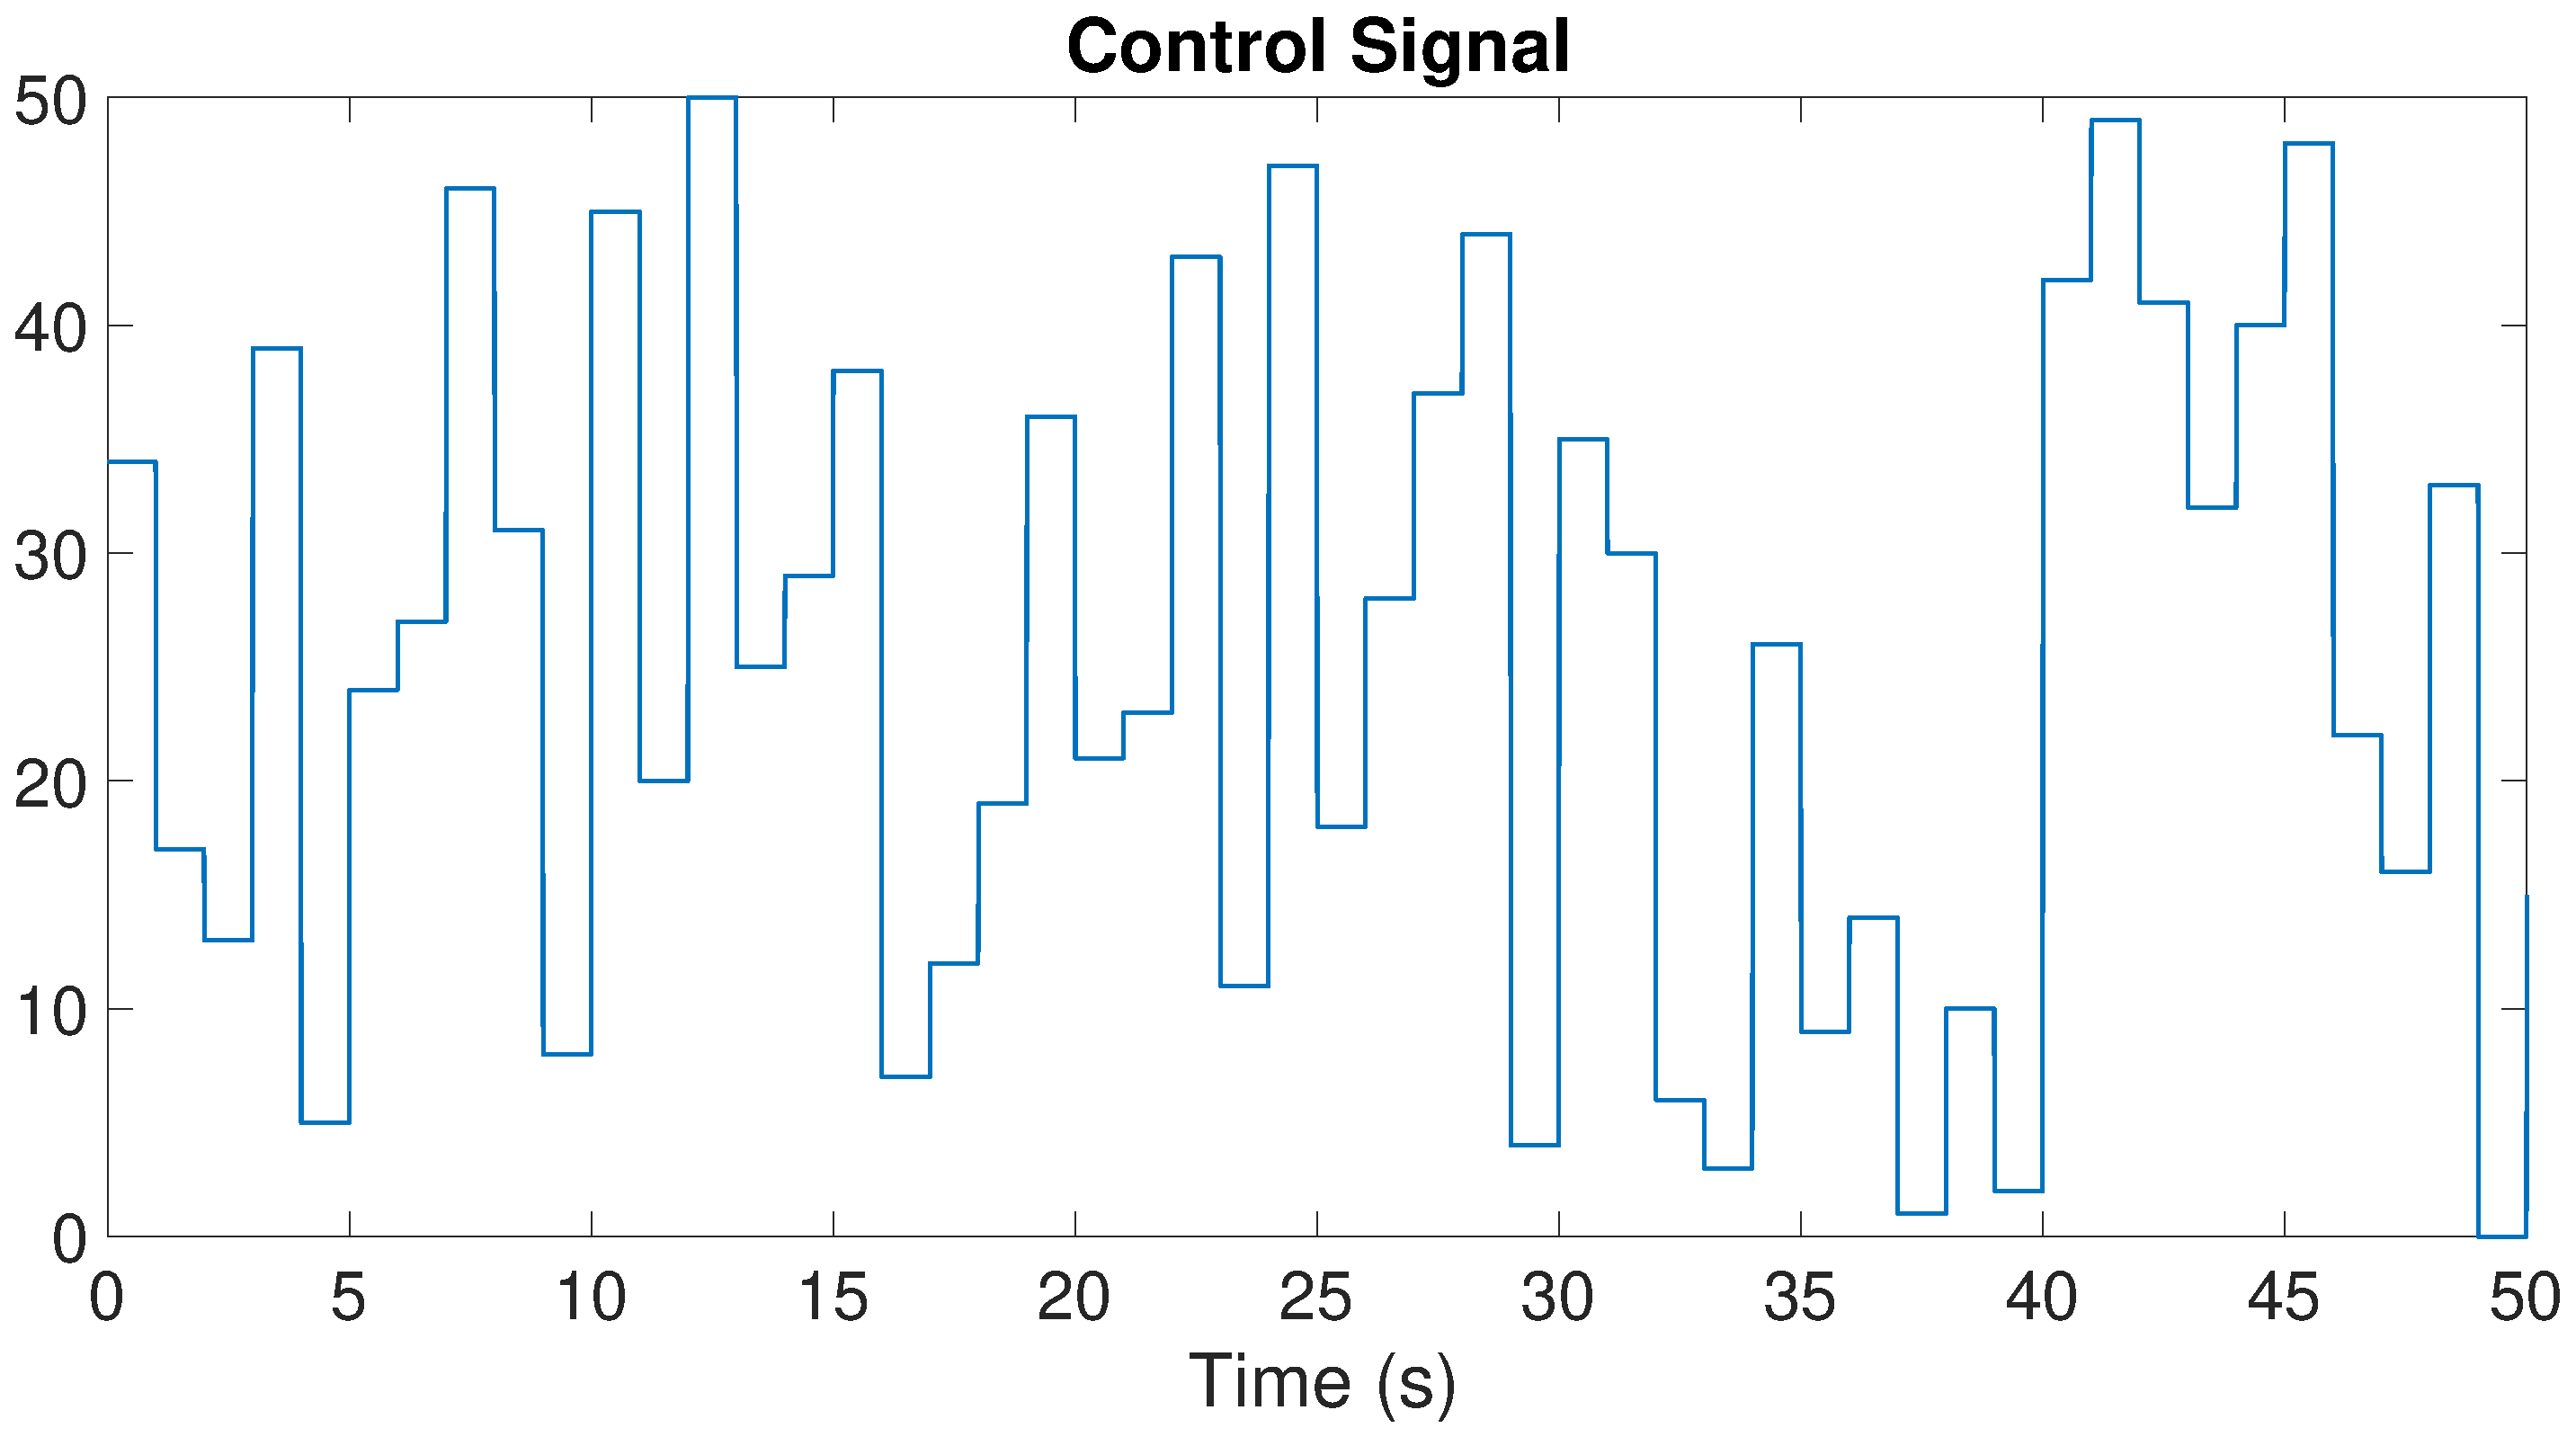
\includegraphics[width=\linewidth]{stair-input-u2}
        \caption{Control Signal.}%
      \end{figure}
    \end{column}%
  \end{columns}
\end{slide}

\begin{slide}{Observer}
  \begin{columns}[c]
    \begin{column}{0.55\textwidth}
      \begin{figure}[ht!]
        \centering
        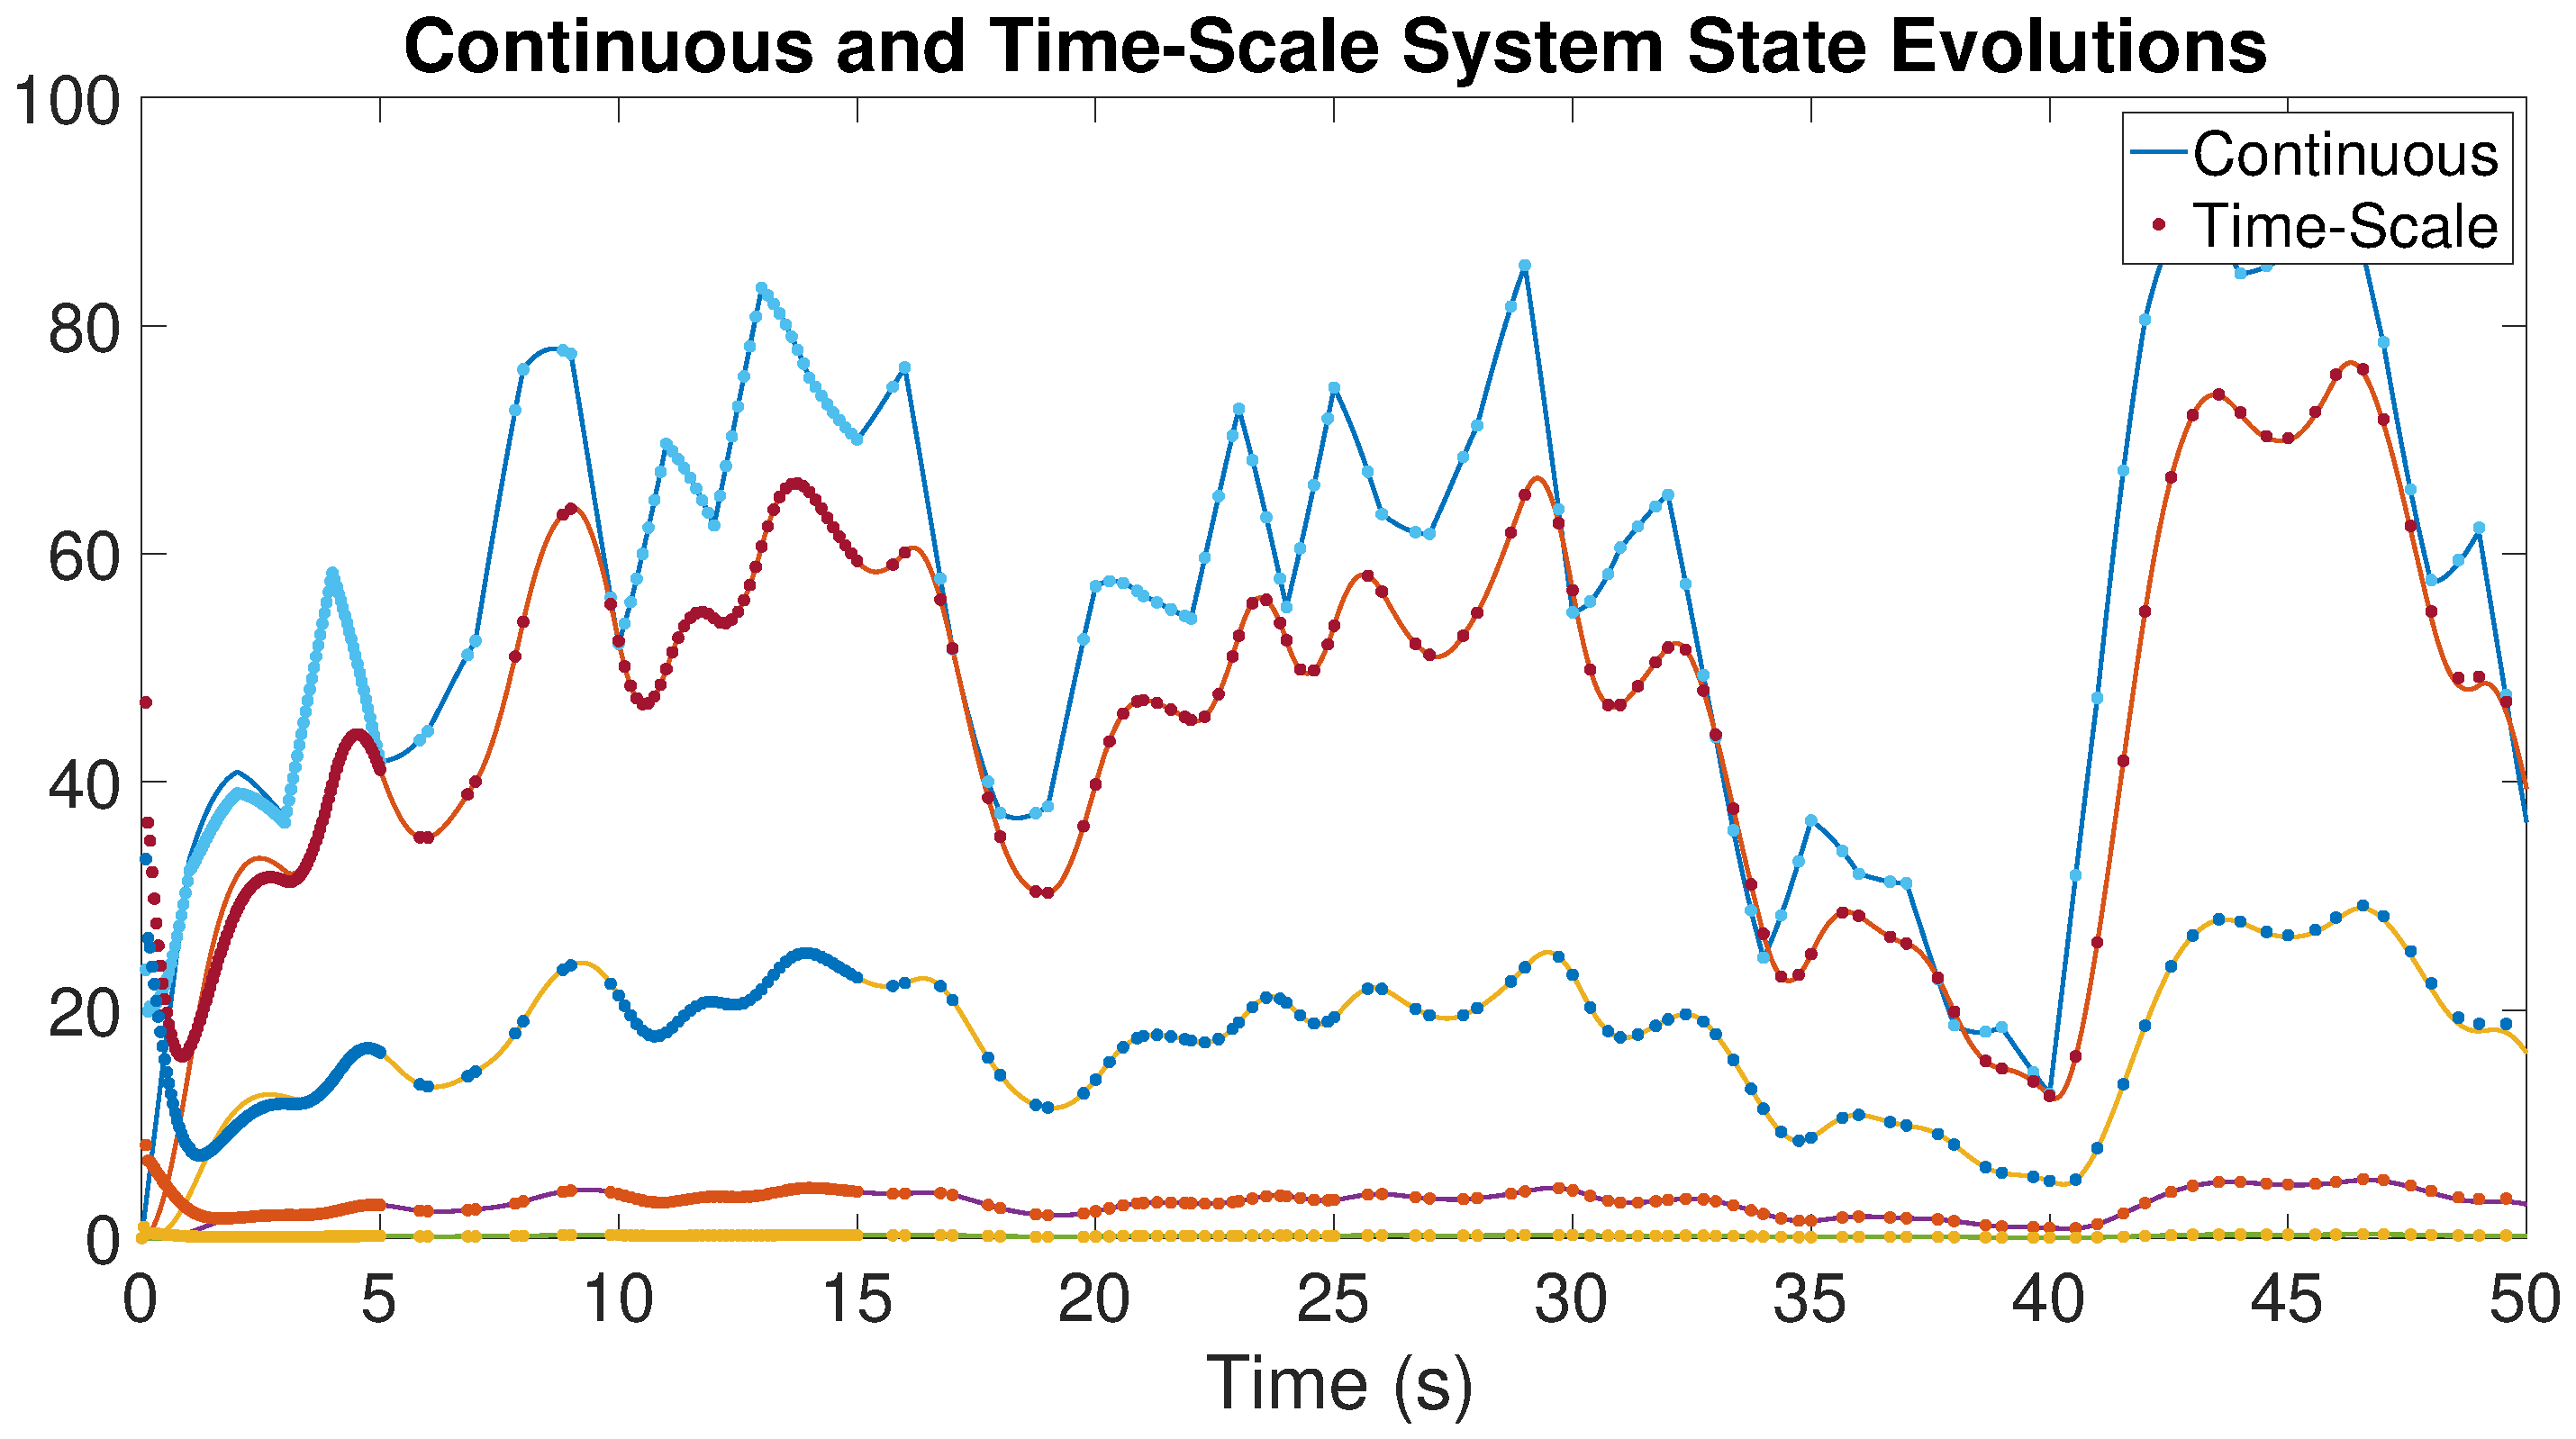
\includegraphics[width=\linewidth]{stair-input2}
        \caption{Observed and system's states.}%
      \end{figure}
    \end{column}%
    \hfill%
    \begin{column}{0.55\textwidth}
      \begin{figure}[ht!]
        \centering
        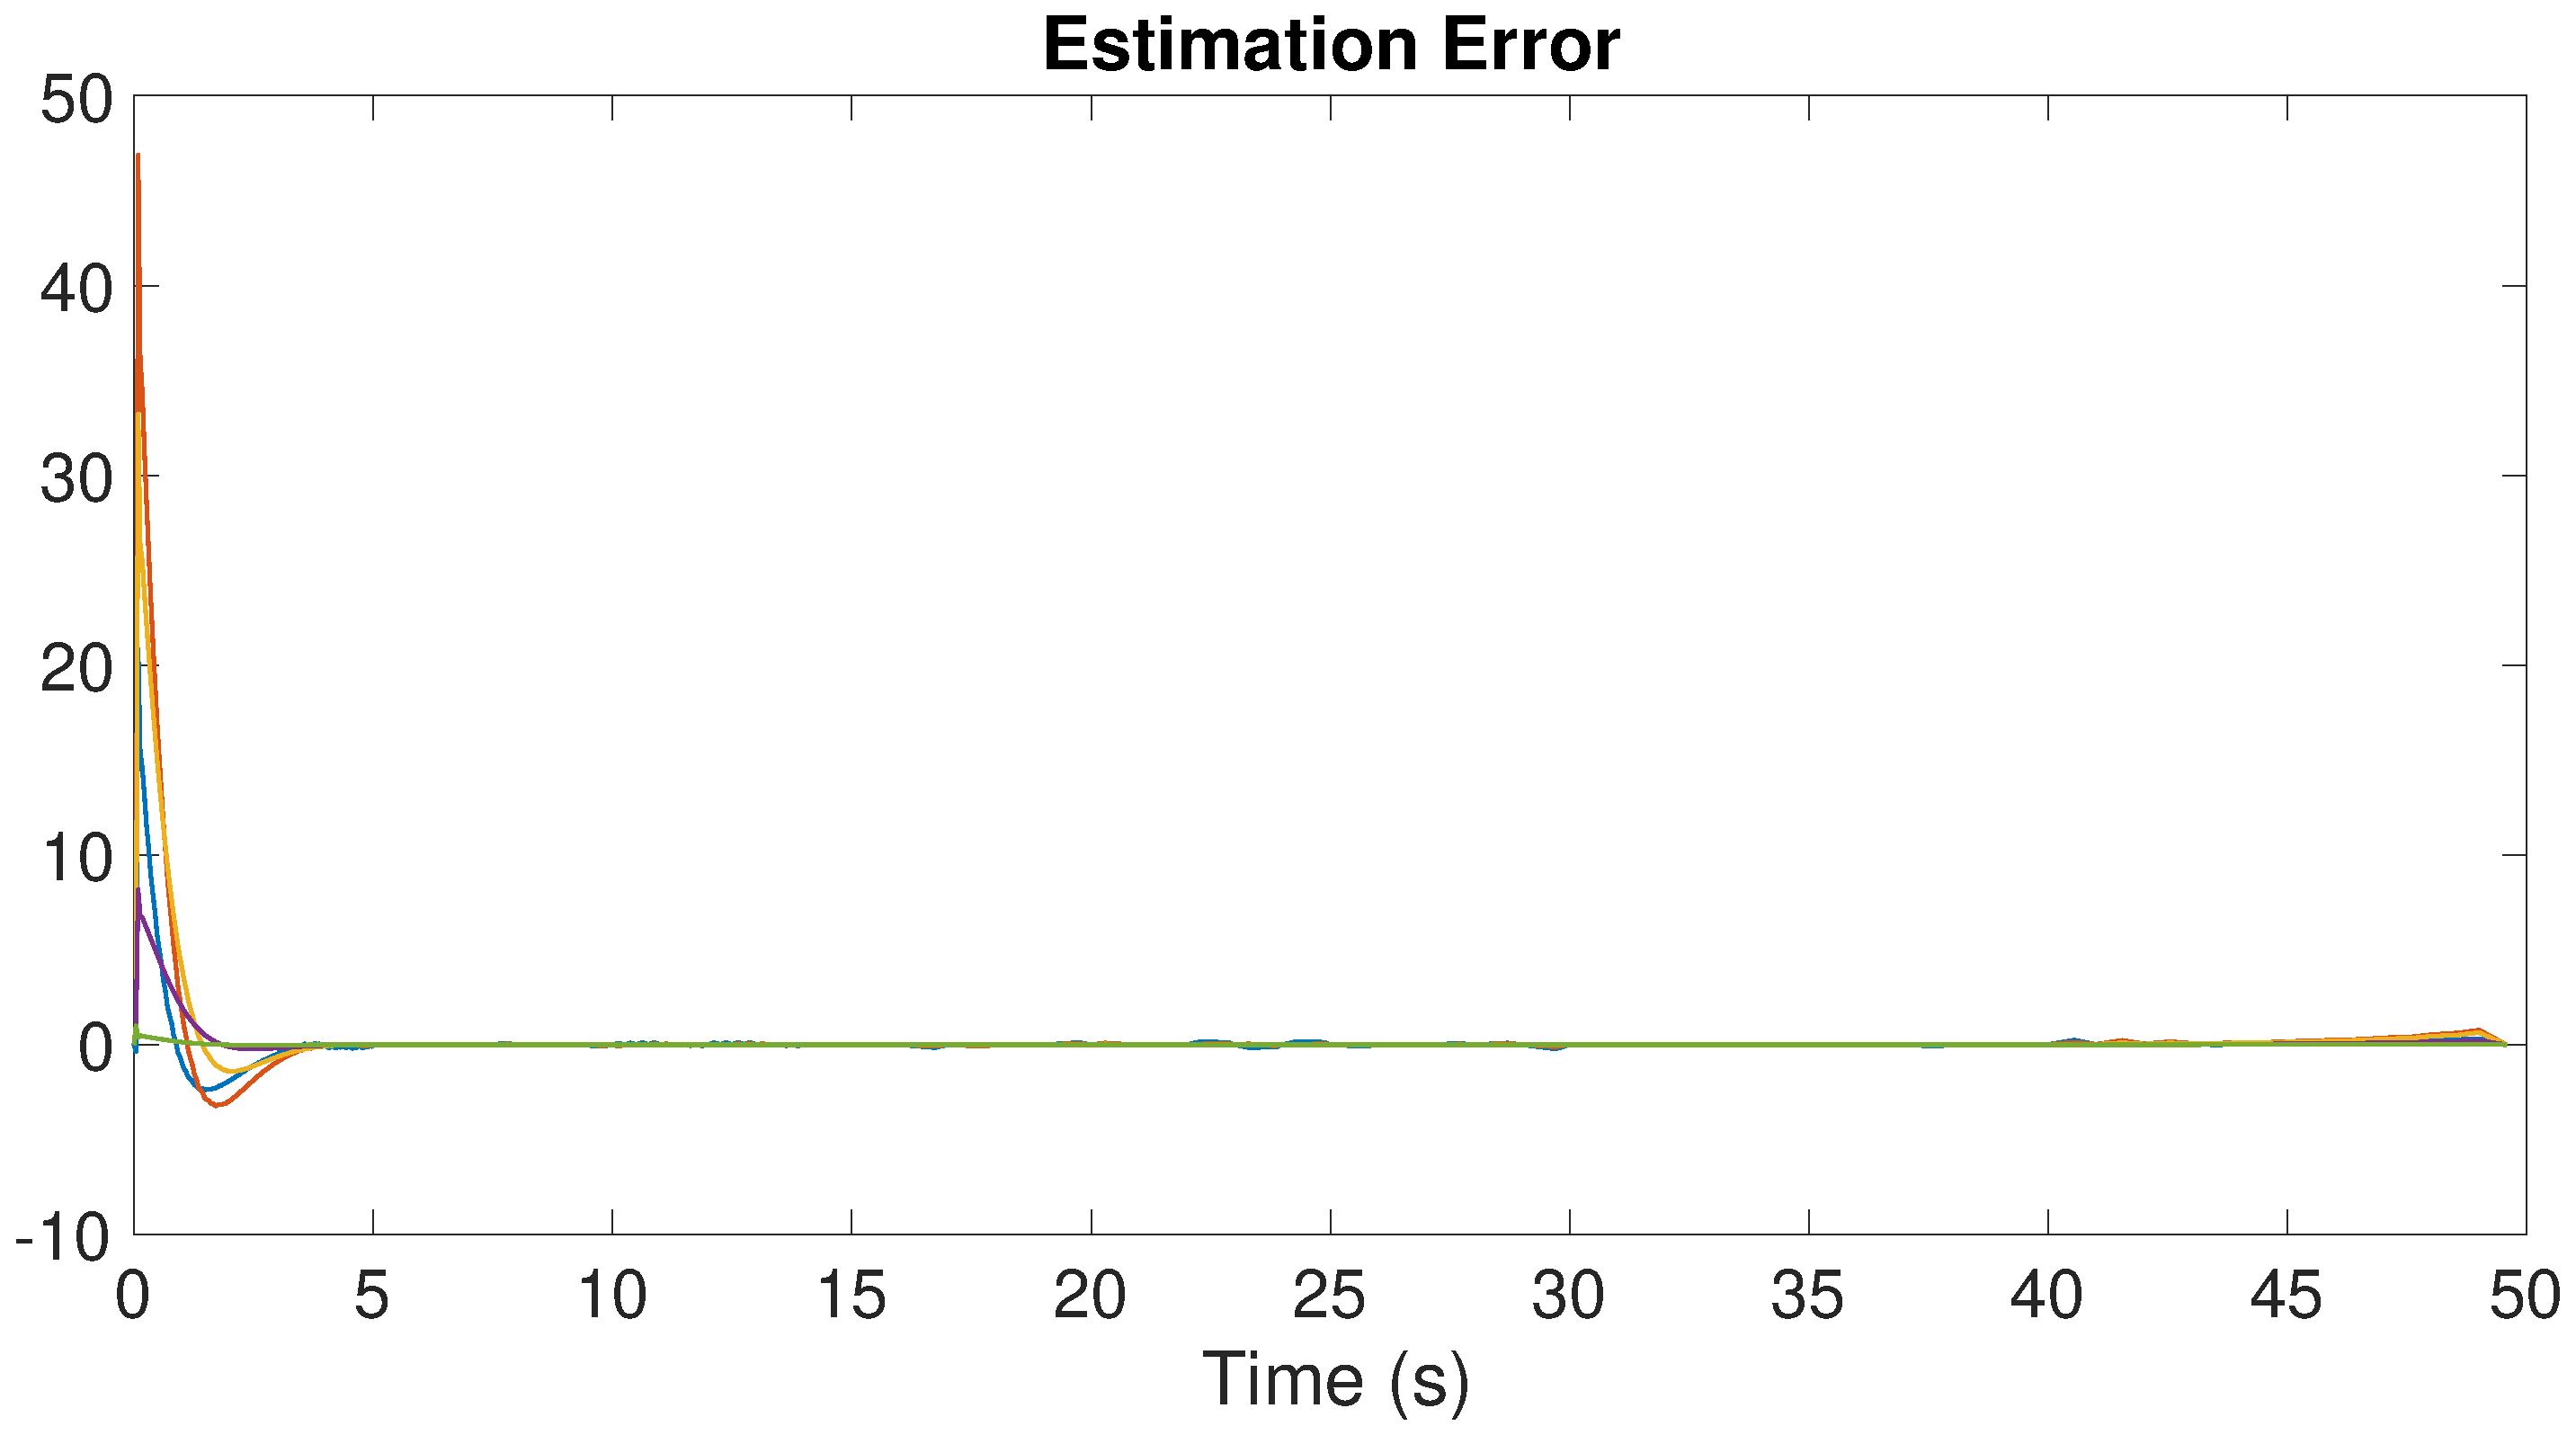
\includegraphics[width=\linewidth]{stair-input-error2}
        \caption{Estimation error.}%
      \end{figure}
    \end{column}%
  \end{columns}
\end{slide}

\begin{slide}{Observer}
  \begin{columns}[c]
    \begin{column}{0.55\textwidth}
      \begin{align}
        \mathcal{A}    & = \begin{bmatrix}
                             -1 & 1  & 0     & 0  & 0  \\
                             -1 & -1 & 1.495 & 0  & 0  \\
                             0  & 0  & -2    & 1  & 0  \\
                             0  & 0  & 0     & -3 & 1  \\
                             0  & 0  & 0     & 0  & -5
                           \end{bmatrix},        \\
        \mathcal{B}    & =\begin{bmatrix}
                            0 \\ 0 \\ 0 \\ 0 \\ 16
                          \end{bmatrix},
        \mathcal{C} = \begin{bmatrix}
                        -5.517 \\ 2.759 \\ 0 \\ 0 \\ 0
                      \end{bmatrix}^{\top},
        \mathcal{D} = 0                                     \\
        \textrm{poles} & = \{-1\pm{}1\imath{}, -2, -3, -5\}
      \end{align}
    \end{column}%
    \hfill%
    \begin{column}{0.55\textwidth}
      \begin{figure}[ht!]
        \centering
        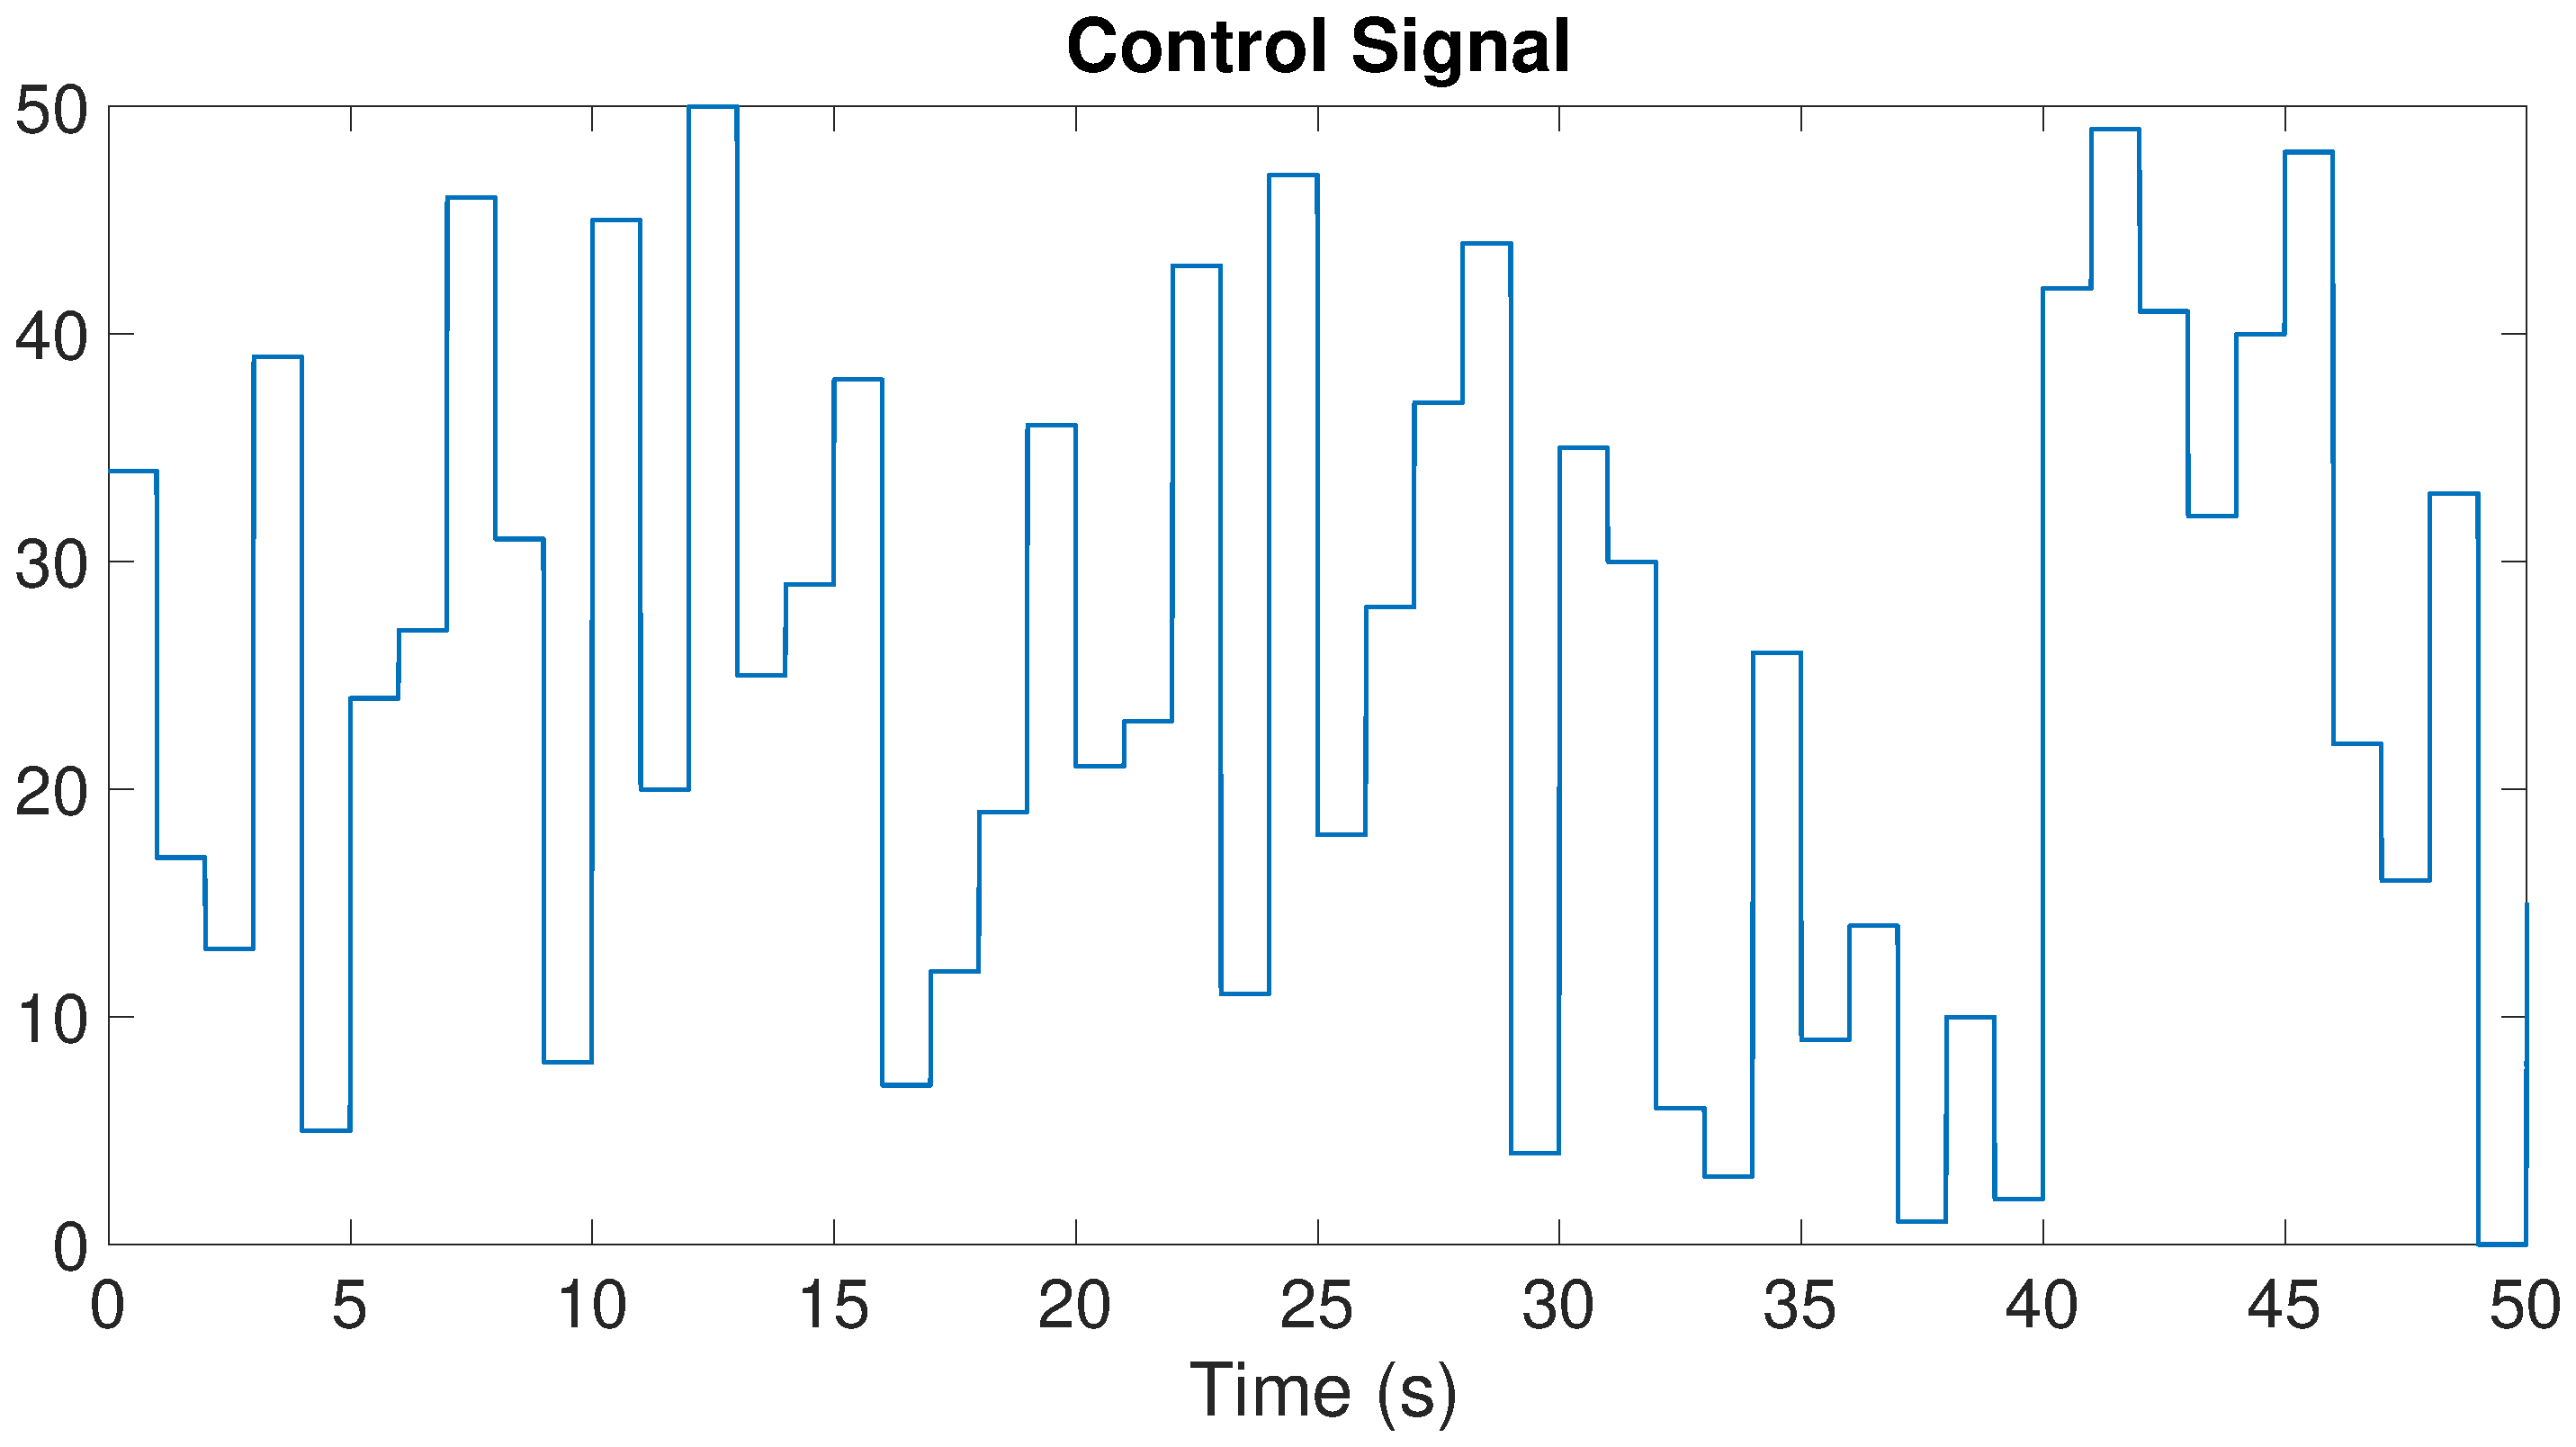
\includegraphics[width=\linewidth]{stair-input-u}
        \caption{Control Signal.}%
      \end{figure}
    \end{column}%
  \end{columns}
\end{slide}

\begin{slide}{Observer}
  \begin{columns}[c]
    \begin{column}{0.55\textwidth}
      \begin{figure}[ht!]
        \centering
        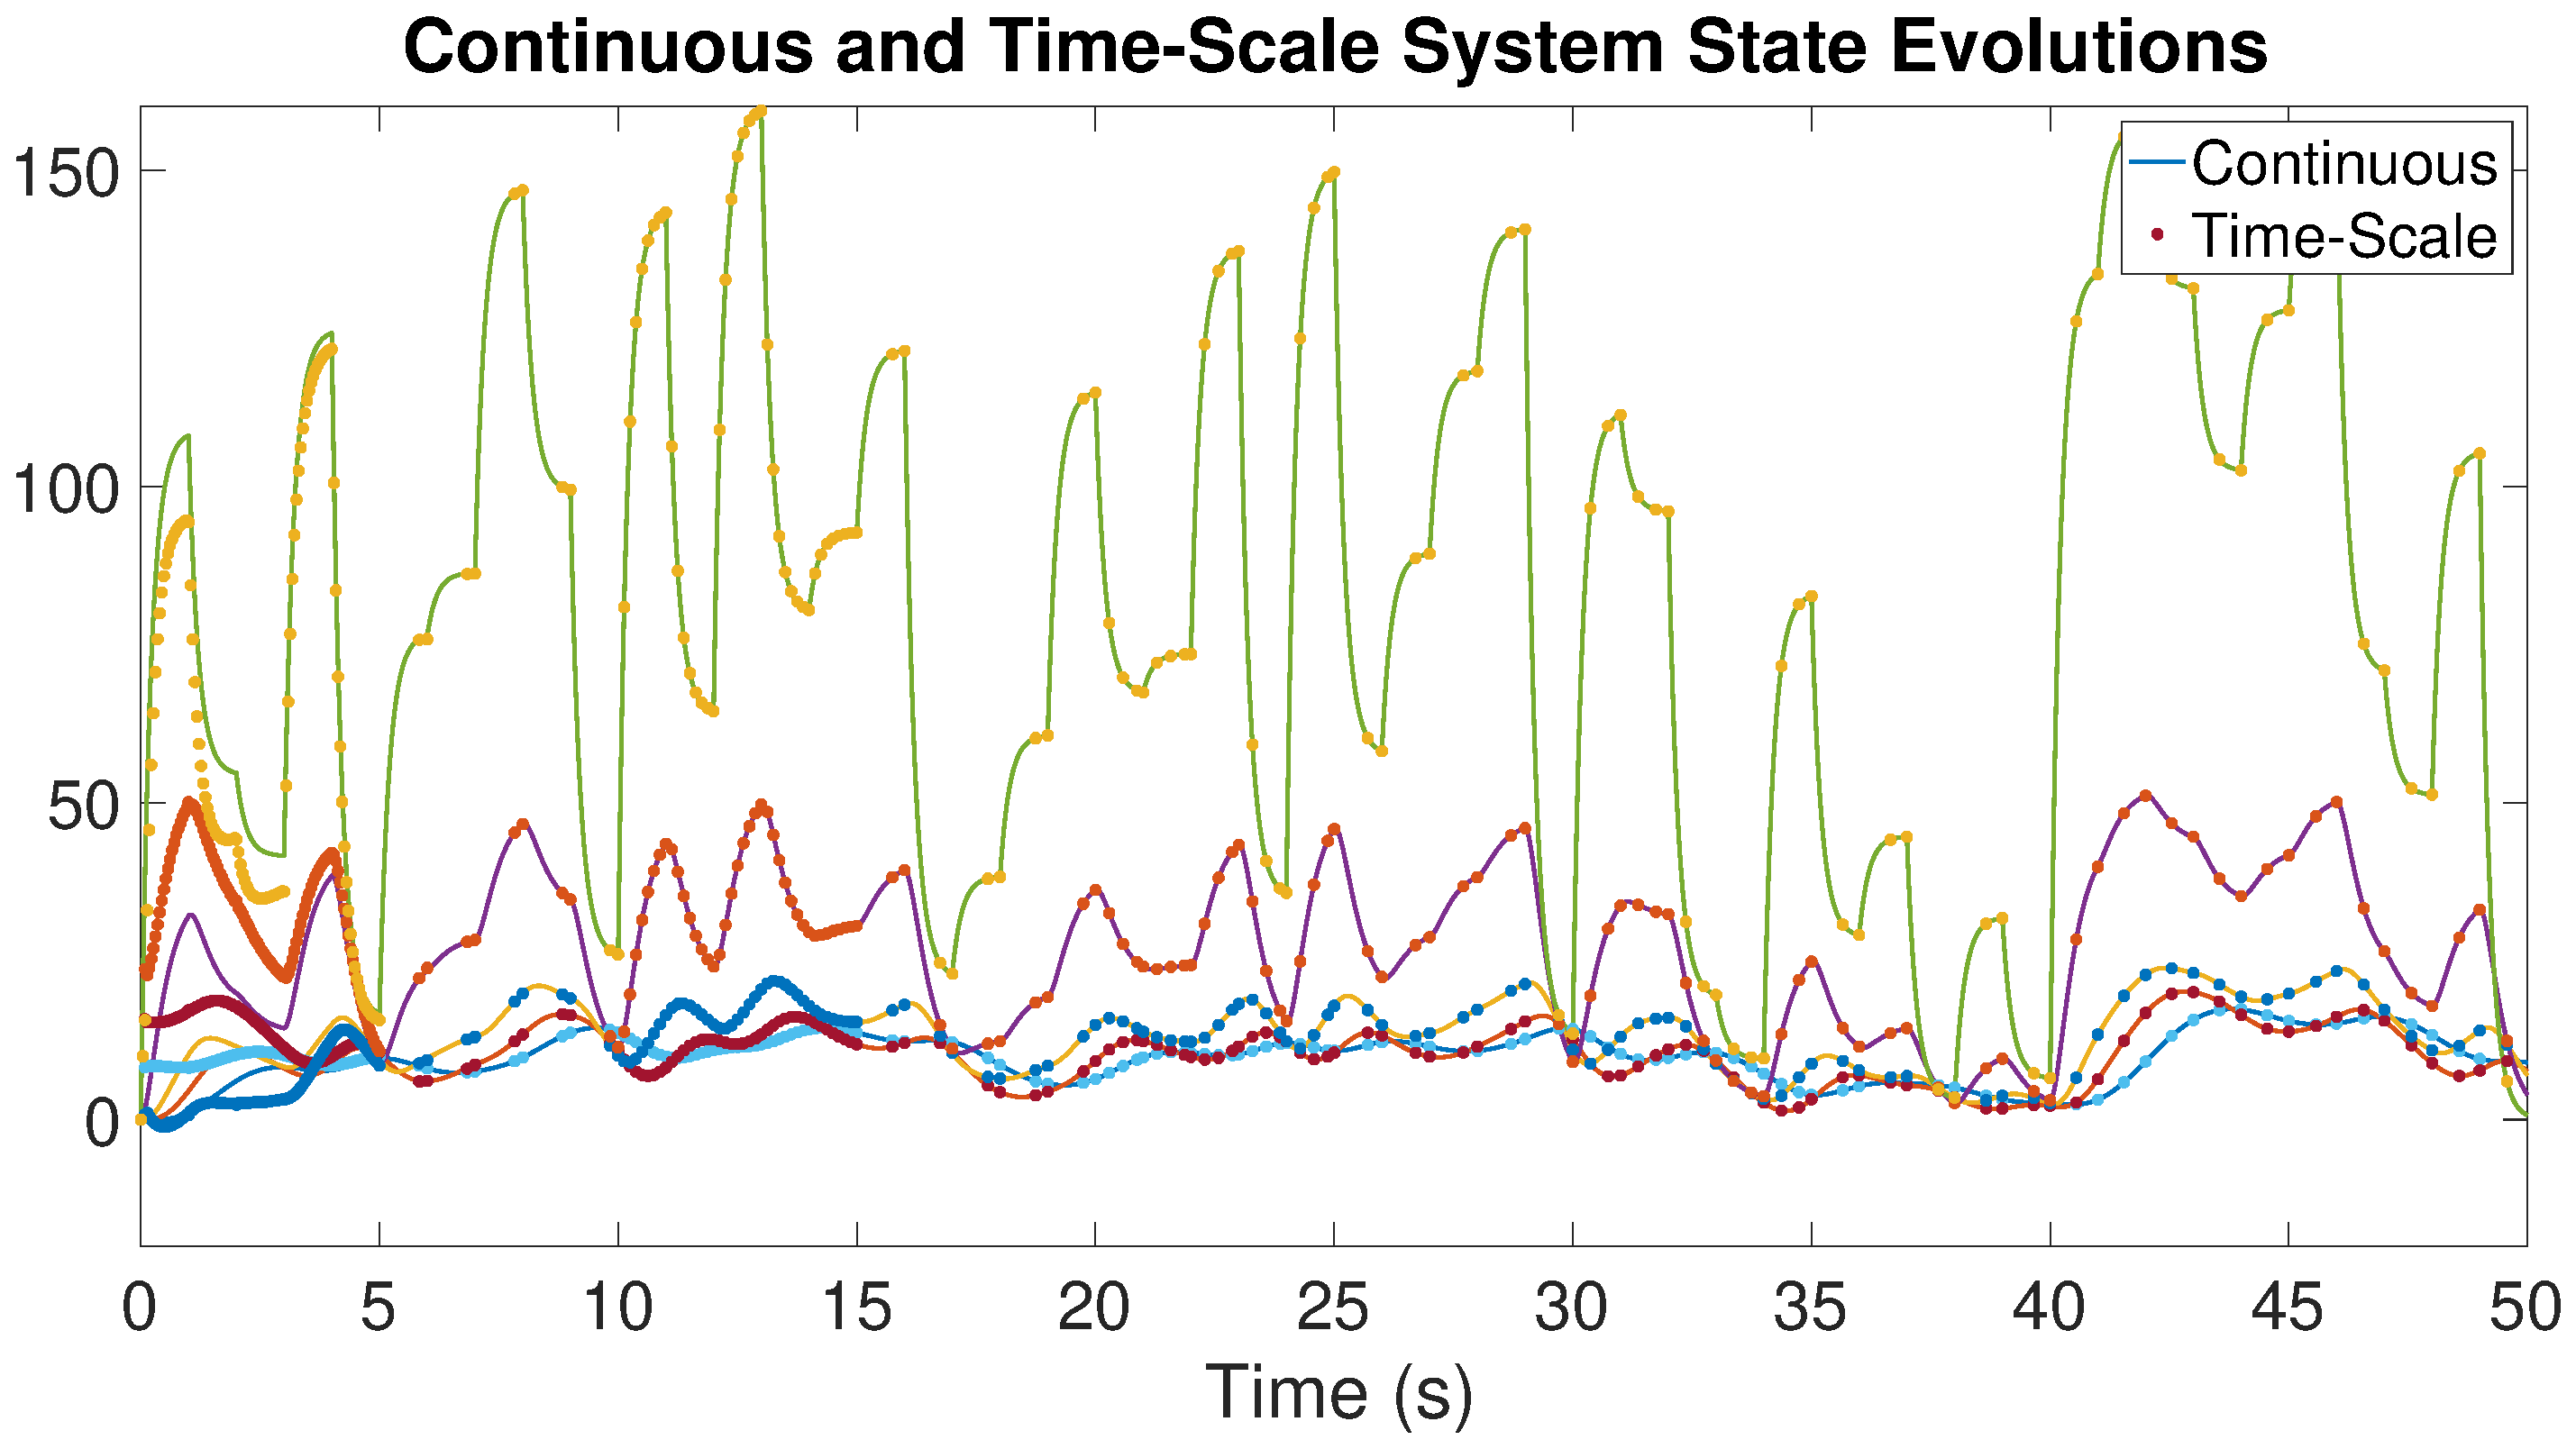
\includegraphics[width=\linewidth]{stair-input}
        \caption{Observed and system's states.}%
      \end{figure}
    \end{column}%
    \hfill%
    \begin{column}{0.55\textwidth}
      \begin{figure}[ht!]
        \centering
        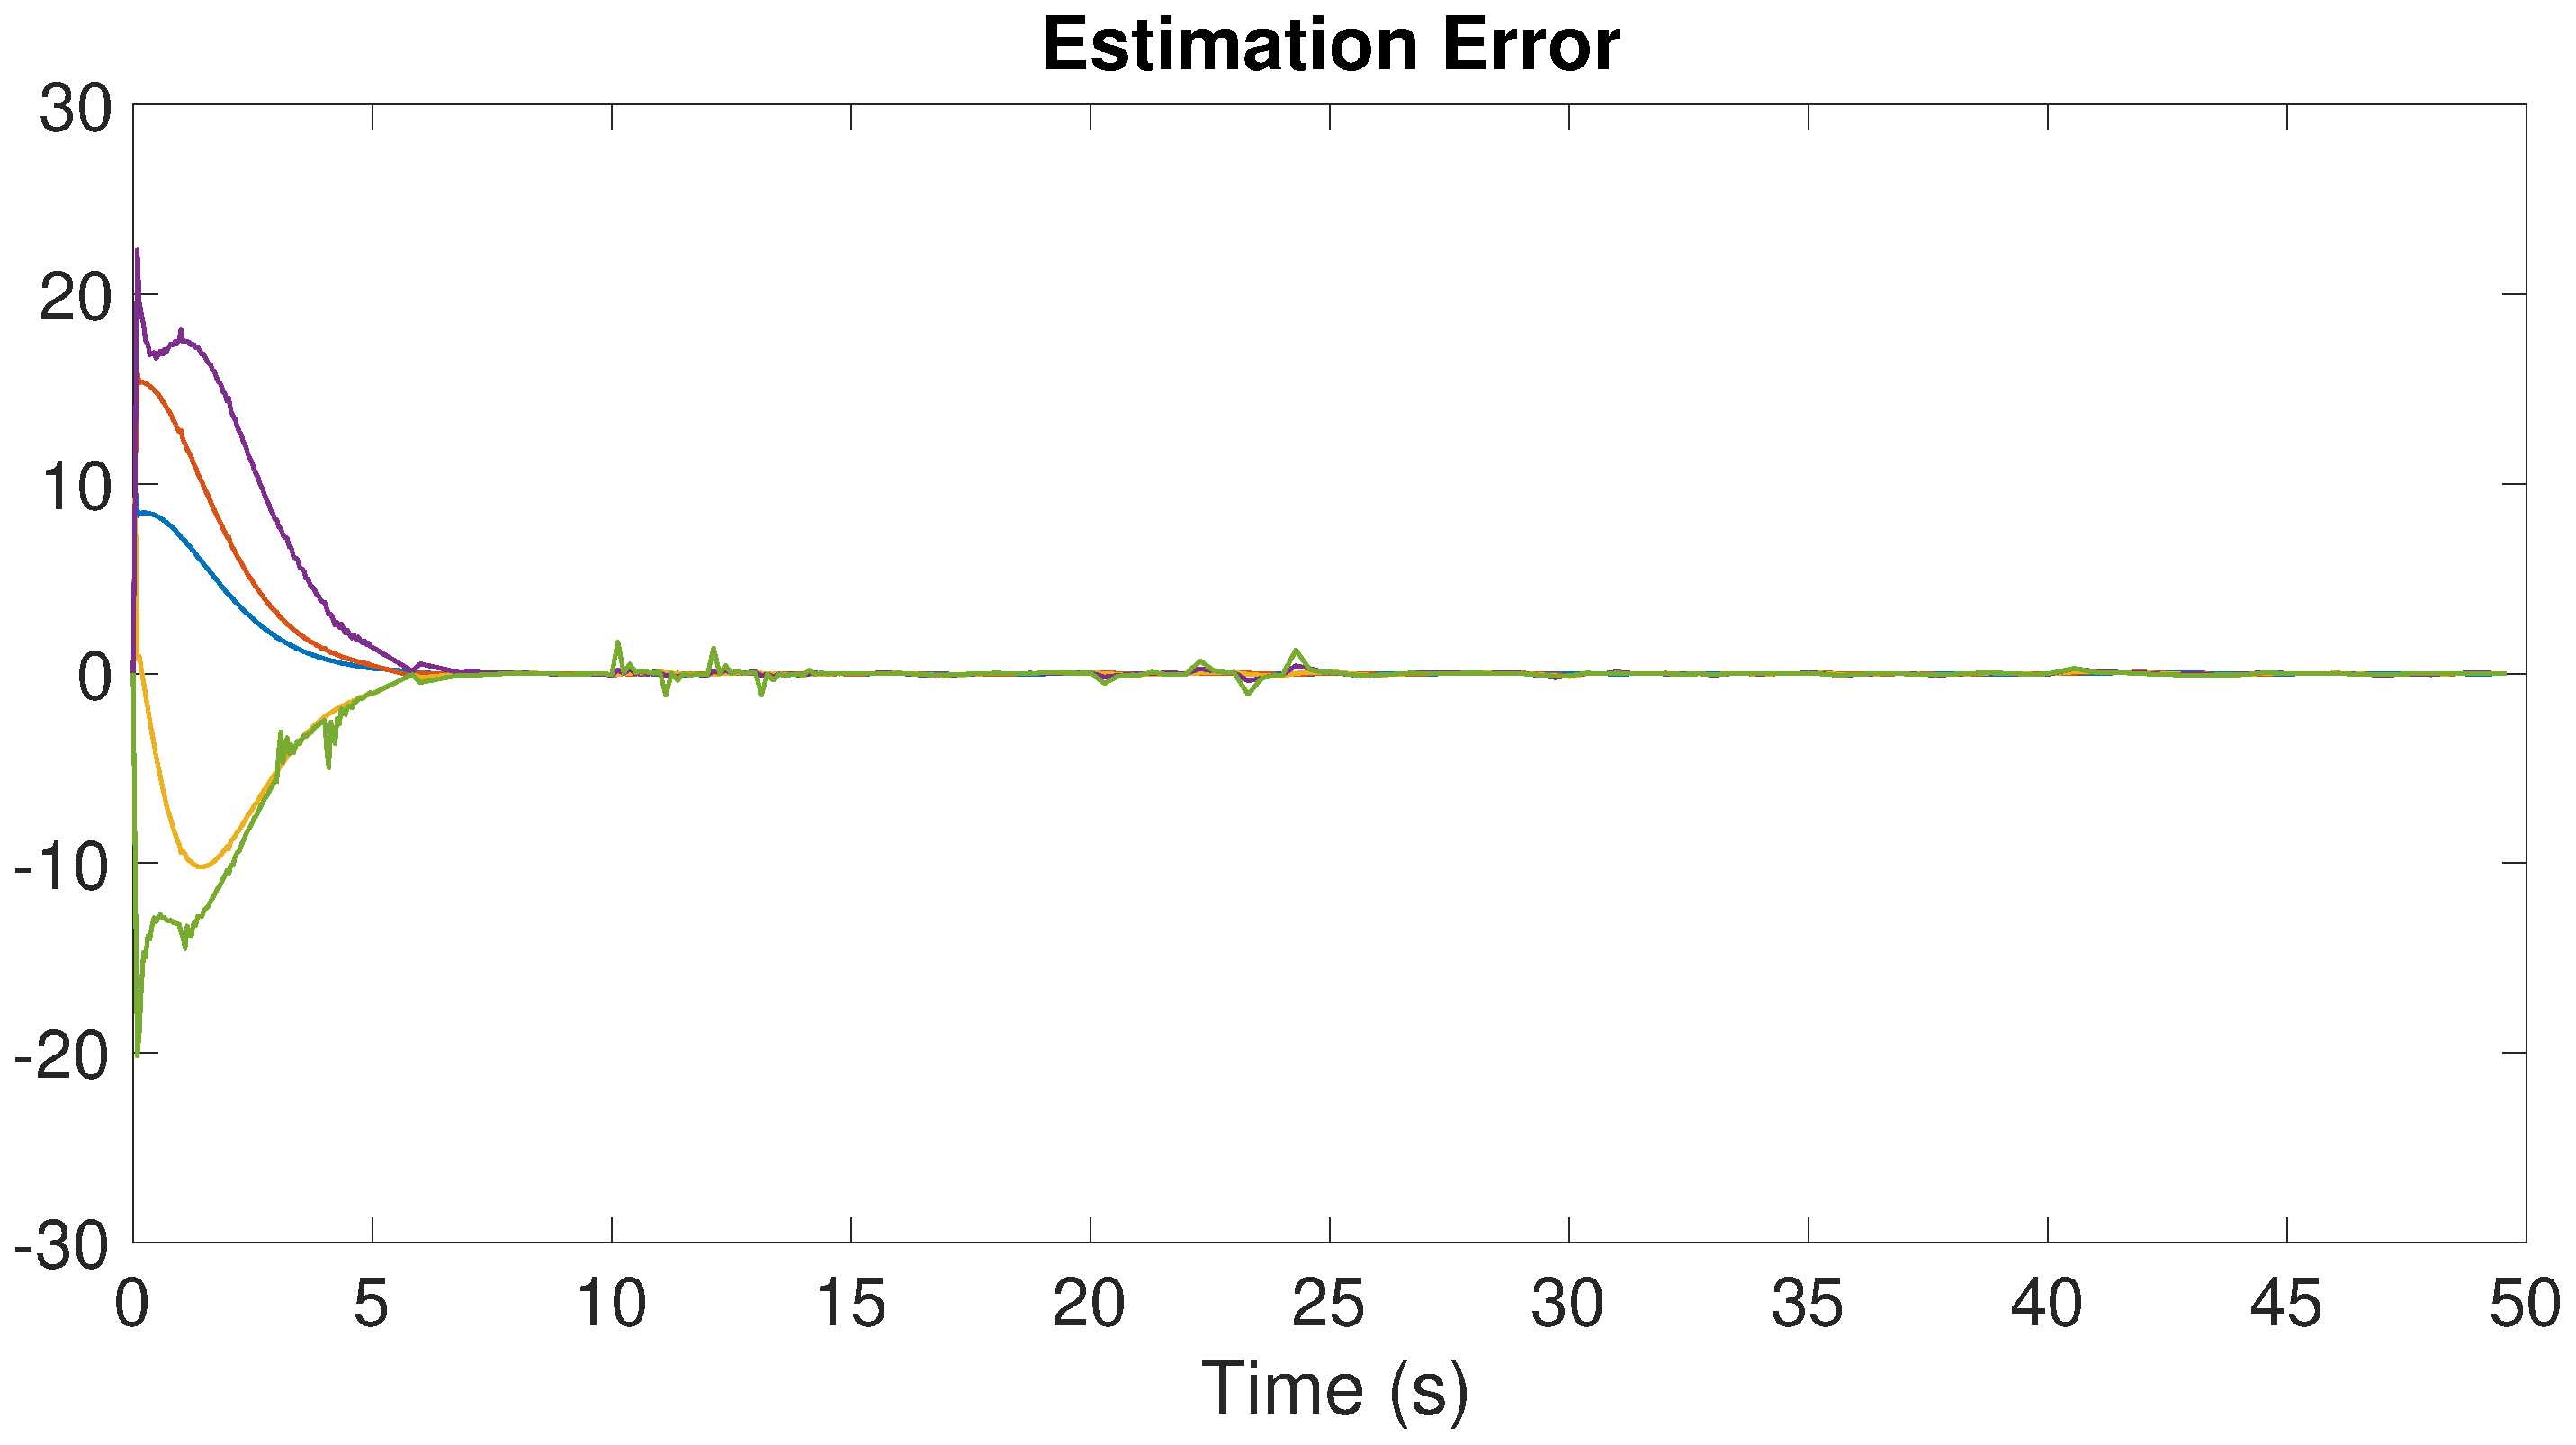
\includegraphics[width=\linewidth]{stair-input-error}
        \caption{Estimation error.}%
      \end{figure}
    \end{column}%
  \end{columns}
\end{slide}

\begin{slide}{Results}
  \begin{columns}[c]
    \begin{column}{0.55\textwidth}
      \begin{figure}[ht!]
        \centering
        \includegraphics[width=\linewidth]{ts-system}
        \caption{Time-scale system's observer with \(\mu=\SI{1}{\second}\).}%
      \end{figure}
    \end{column}%
    \hfill%
    \begin{column}{0.55\textwidth}
      \begin{figure}[ht!]
        \centering
        \includegraphics[width=\linewidth]{ts-system2}
        \caption{Time-scale system's observer with \(\mu=\SI{0.75}{\second}\).}%
      \end{figure}
    \end{column}%
  \end{columns}
\end{slide}

% !TeX root = document.tex
% !TeX encoding = UTF-8 Unicode

\subsection{Partial Conclusion}%
\label{subsec:ts-conclusion}

\begin{slide}{Partial Conclusion}
  \begin{itemize}
    \item The formulation is straightforward, optimization based and extendable.
    \item The graininess \(\mu\) can change randomly to avoid attack vectors
          which may also affect the time-scale system. Better yet, techniques as
          the Game Theory's Moving Target can give the best strategies to
          changing its value.
    \item A future work may try to find bounds for the complex-valued poles.
    \item The next step is to make a Functional-Time-Scale observer, and/or a
          distributed one.
  \end{itemize}
\end{slide}


\begin{slide}{}
  \usebeamercolor{frametitle}
  \vspace*{\fill}
  \begin{center}
    \textcolor{fg}{\Large{Merci pour votre attention.}}
  \end{center}
  \vspace*{\fill}
\end{slide}

\begin{slide}[allowframebreaks]{References}
  \nocite{*}
  \printbibliography{}
\end{slide}
\end{document}
